\section{}
\subsection{}
{A beam of negligible mass has two masses of M attached as shown. Estimate the lowest natural frequency using Rayleigh's Quotient. Assume}
\begin{align*}
    \mathbb{Y}(x) &= A(x - \frac{2L}{3})(x + \frac{2L}{3}) \\
    &= A(x^2 - \frac{4L^2}{9})
\end{align*}
\begin{figure}[H]
    \centering
    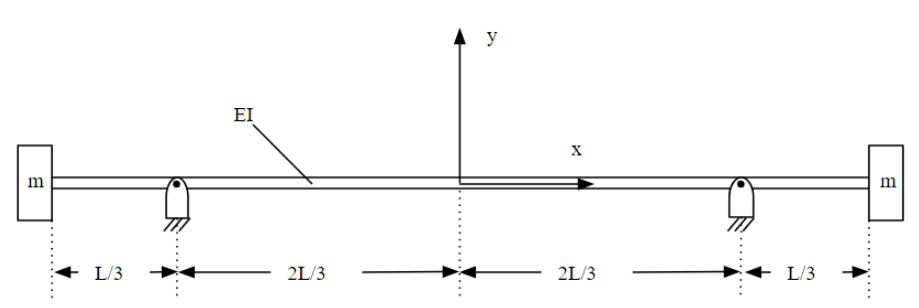
\includegraphics[width=0.6\linewidth]{Questions/Figures/Q3 Problem Diagram.png}
\end{figure}
Recall the Rayleigh's Quotient for continuous systems:
\begin{align*}
    p^2 &= \displaystyle\frac{\displaystyle \int_{-L}^{L} EI \left(\frac{d^2 \mathbb{Y}}{dx^2}\right)^2 dx + \displaystyle\sum_{i = 1}^{s} k_i \left(\mathbb{Y}(x_i)\right)^2}{\displaystyle \int_{-L}^{L} \rho A \left(\mathbb{Y}\right)^2 dx + \displaystyle\sum_{j = 1}^{n} m_j \left(\mathbb{Y}(x_j)\right)^2}
\end{align*}
Let us evaluate convenient quantities for the given beam:
\begin{align*}
    \frac{d^2 \mathbb{Y}}{dx^2} &= 2A \\
    \mathbb{Y}(-L) &= A(L^2 - \frac{4L^2}{9}) = \frac{5AL^2}{9} \\
    \mathbb{Y}(L) &= A(L^2 - \frac{4L^2}{9}) = \frac{5AL^2}{9}
\end{align*}
Then the terms of the Rayleigh's Quotient become:
\begin{align*}
    \int_{-L}^{L} EI \left(\frac{d^2 \mathbb{Y}}{dx^2}\right)^2 dx &= 4EIA^2 \int_{-L}^{L} dx \\
    &= 8EIA^2 L \\
    \int_{-L}^{L} \cancelto{\text{negligible}}{\rho} A \left(\mathbb{Y}\right)^2 dx &= 0 \\
    m_{1} \left(\mathbb{Y}(-L)\right)^2 &= m \frac{25 A^2 L^4}{81} \\
    m_{2} \left(\mathbb{Y}(L)\right)^2 &= m \frac{25 A^2 L^4}{81} 
\end{align*}
Therefore, the Rayleigh's Quotient for the given beam is:
\begin{align*}
    p^2 &= \frac{8 EIA^2L}{m\frac{50 A^2 L^4}{81}} \\
    &= \frac{324 E I}{25 m L^3}
\end{align*}
And the lowest natural frequency is:
\begin{align*}
    \Aboxed{p &= \sqrt{\frac{324}{25}} \cdot \sqrt{\frac{E I}{m L^3}}} 
\end{align*}

\subsection{}
\textit{To stiffen the system a section is added to increase the natural frequency by 25\%. Using the same trial function as above, estimate the parameter $\alpha$ to determine the length of the stiffened section.}

The denominator of the Rayleigh's Quotient is the same as before. We only need to evaluate the numerator for the stiffened system. Using symmetry, 
\begin{align*}
    2 \left[\int_{0}^{\alpha L} 3 EI \left(\frac{d^2 \mathbb{Y}}{dx^2}\right)^2 dx + \int_{\alpha L}^{L} EI \left(\frac{d^2 \mathbb{Y}}{dx^2}\right)^2 dx\right] &= 2EI \left[3 \int_{0}^{\alpha L} 4A^2 dx + \int_{\alpha L}^{L} 4A^2 dx\right] \\
    &= 2EI \left[12A^2 \alpha L + 4A^2 (1 - \alpha) L\right] \\
    &= 8 E I A^2 L (3 \alpha + 1 - \alpha) \\
    &= 8 E I A^2 L (2 \alpha + 1)
\end{align*}
The Rayleigh's Quotient for the stiffened system is then:
\begin{align*}
    p_2^2 &= \frac{8 E I A^2 L (2 \alpha + 1)}{m \frac{50 A^2 L^4}{81}} \\
    &= \frac{324 E I (2 \alpha + 1)}{25 m L^3}
\end{align*}
Since we want $p_2 = 1.25 p_1$, we have:
\begin{align*}
    1.25^2 p_1^2 &= \frac{324 E I (2 \alpha + 1)}{25 m L^3} \\
    \frac{25}{16} \cdot \frac{324 E I}{25 m L^3} &= \frac{324 E I (2 \alpha + 1)}{25 m L^3} \\
    \frac{25}{16} &= 2 \alpha + 1 \\
    \Aboxed{\alpha &= \frac{9}{32}}
\end{align*}

